%
\section{Laundry database library}

Most of the project subtask groups decided to use one programming language to make it easier to work together. Sometimes different languages can be difficult to connect and operate together. Therefore it was decided to use one object oriented language - C\#. As we know C\# is a one of the new generation languages, which provides a lot of advanced features like strong type checking, a garbage collector, robustness and durability. \\ This kind of language makes it easier to develop programs like this subtask, because there is no need for taking care of low level features like memory allocation or lost pointers, since low level design is not essential for this subtask. This kind of language can decrease the duration of the development process and increase code efficiency. \\

All data were stored in MySQL database. Many of the other subtasks would need an access to it and that is why we decided to create a library providing access for any subtask to use. The design requirement is to create a general library which has the features of:  reliability, easy maintenance and simple to use.

\subsection{Design phase}

Due to the mentioned requirements and features it was decided to create a DLL (dynamic link library). The library inside has two classes:

\begin{itemize}
	\item MySQLConnection \textendash database connector which responsible for connection to database and send/receive queries.
	\item Functions \textendash general library for laundry database.
\end{itemize}

\begin{figure}[h]
	\centering
		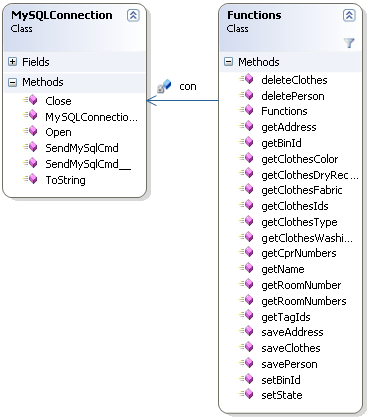
\includegraphics[scale=0.7]{classLibrary}
	\caption{Class library of the database connection}
	\label{fig:planning}
\end{figure}

\newpage
\subsection{Implementation}

Software development was related to the unified process (UP) - iterative incremental process.  Iterative incremental process model \cite{bib5} was used during the implementation.  
The project was created using the class Library in Microsoft Visual C\# known as the .NET 3.5 framework. The database connection was included by adding MySQL Connector Net 1.0.10 into references. The created library was included into the other/new projects (Console or Win or something else) and the library was utilized. For example the library was  inserted into a console project, a connection to database was created, shown in the figure \ref{fig:connectionToData}. After a successful connection to the library class functions are usable and enables management of the laundry database.

\begin{figure}[h]
	\centering
		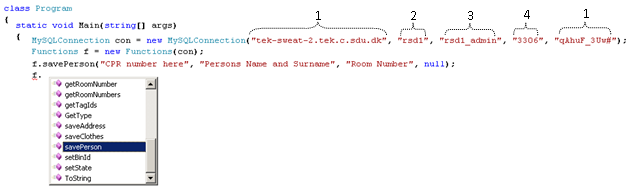
\includegraphics[scale=0.7]{connectionToData}
	\caption{Connection to database server and save new person}
	\label{fig:connectionToData}
\end{figure}

Numbers explaining the database connection parameters:

\begin{enumerate}
	\item IP address or domain
	\item Database name
	\item User Id
	\item Port number
	\item Password
\end{enumerate}

Class functions are used to create instances of the MySQLConnection library, and through the variable f all the created methods can be called. The figure \ref{fig:exampleSavePerson} shows an example of the creation of a new person. Shown on the figure, there is used methods to send queries to the database. New CPR is inserted into the person table by query: “INSERT INTO Person (CPR) Values (‘1234567890’)”.

\begin{figure}[h]
	\centering
		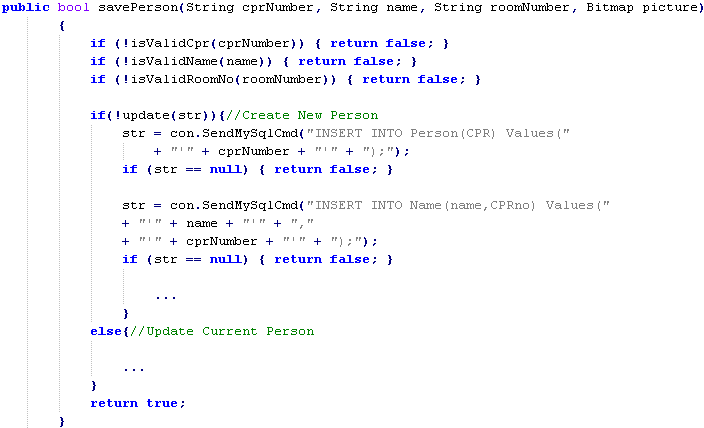
\includegraphics[scale=0.7]{exampleSavePerson}
	\caption{Example of save person method}
	\label{fig:exampleSavePerson}
\end{figure}